\section{Lessons Learned}\label{sec:lessons_learned}

After over 6 months of weekly meetings, the authors have identified
aspects of the Dojo that went well, aspects that went less well and
aspects that still are puzzles to understand.

Since the sessions are being held, the authors could identify what
practices and rules went well (Subsection \ref{ssub:well}) but also
found out that some things work less well (\ref{ssub:less_well}) than
expected. Finally, applying the practice to different audiences and in
different contexts, the authors discovered some unaddressed issues
(\ref{ssub:puzzles}).

\subsection{What went well?}\label{ssub:well}

\subsubsection{Retrospectives and action items}

As described in the previous section, every meeting is ended with a
short retrospective. The participants receive red and yellow sticky
cards and write positive and negative aspects of the session that just
ended. In the begining, the group followed a simple retrospective
format, asking ``What worked well?'' for positive aspects and ``What
can be improved?'' for negative aspects. These questions led people to
write items about the process used for the meetings, such as when to
choose the problem, when to change the programming language, what
laptop to use, etc. This kind of feedback helped improve the Sao Paulo
\emph{Coding Dojo} itself, and to reach the process described in
\ref{subsec:dojosp}.

\begin{figure}[htp]
\centering
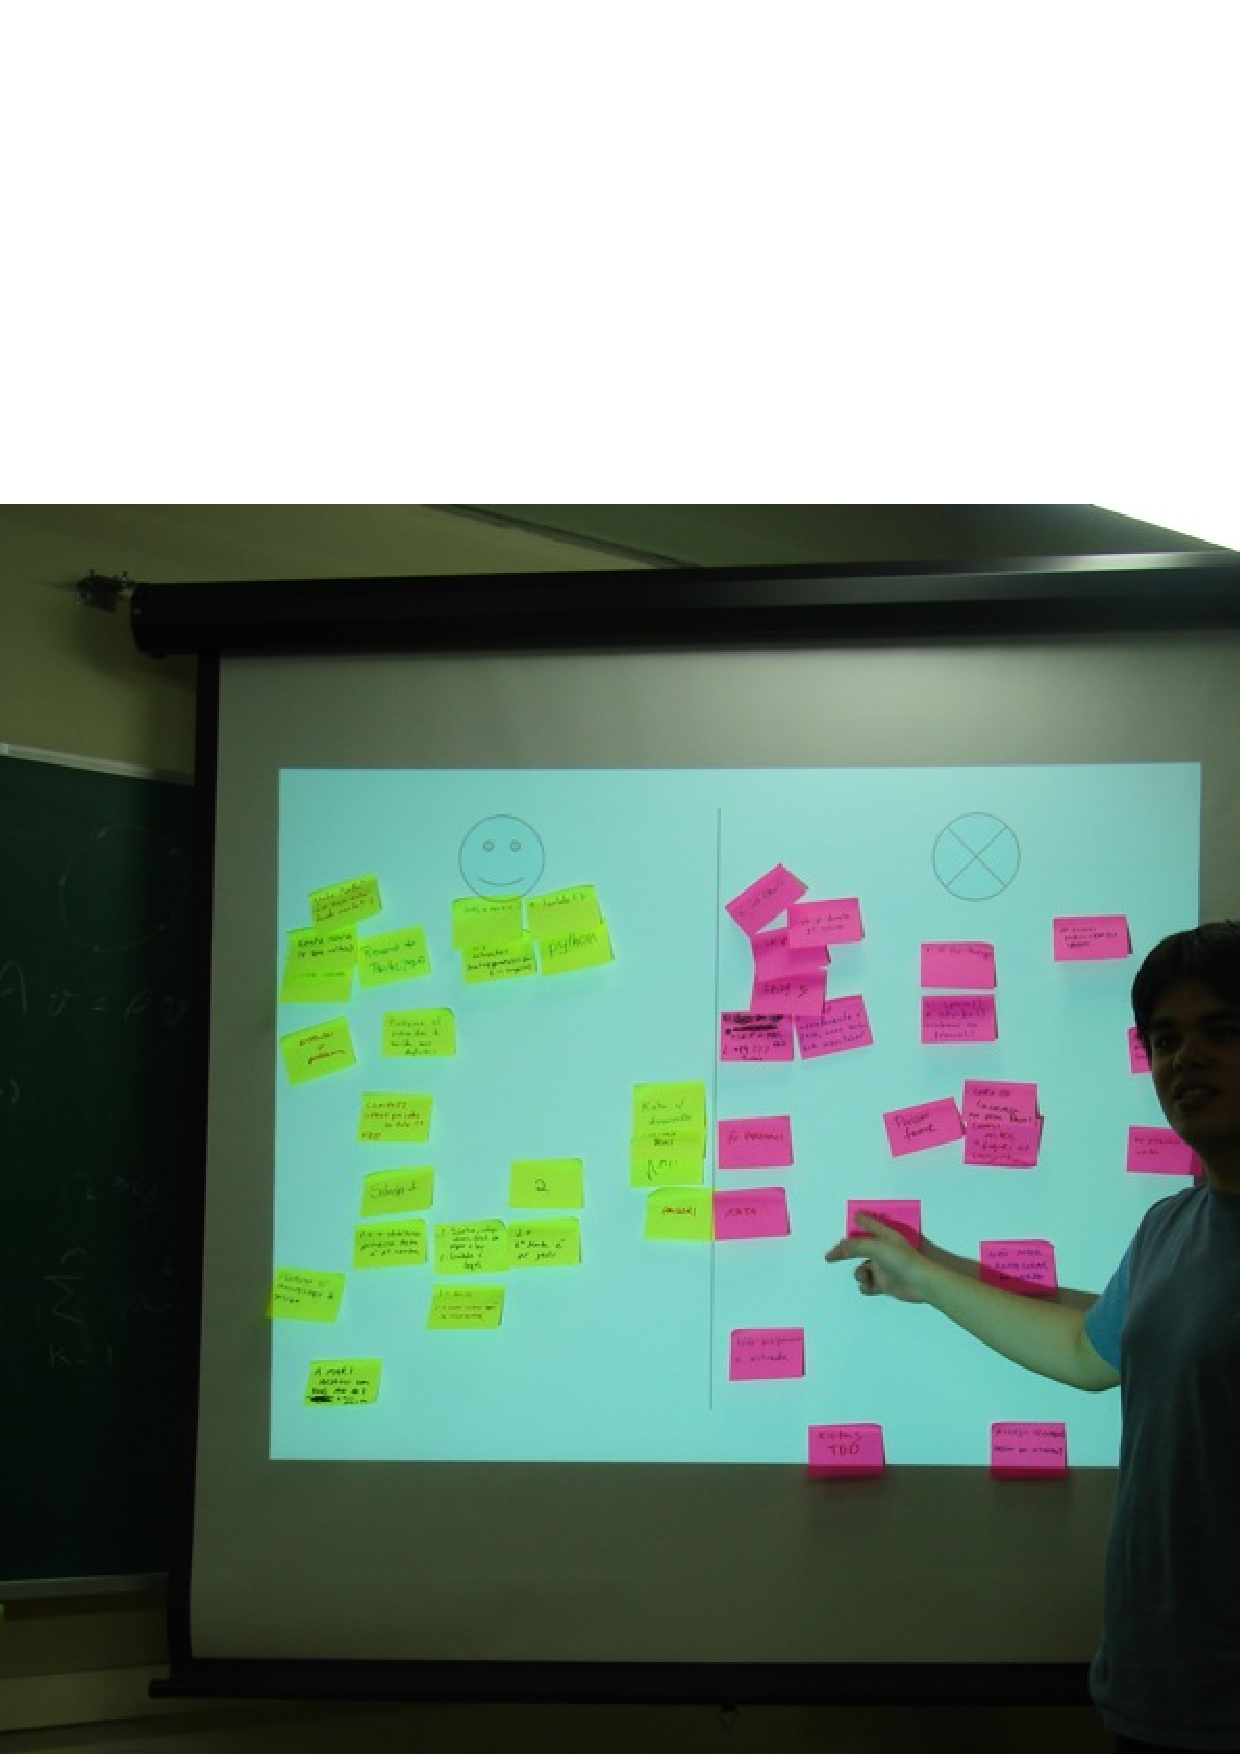
\includegraphics[width=\columnwidth]{retrospective}
\caption{Conducting the retrospective}\label{fig:retrospective}
\end{figure}

After some time, the retrospective format changed to reflect the
objetives of the \emph{Coding Dojo}. Now participantes are asked to
think about the following questions:

\begin{itemize}
\item \textbf{``What have we learned?''}: Reflecting and discussing
  what was learned is an effective way to make learning an active
  process and to verify that the session met its goals.
\item \textbf{``What has hindered learning?''}: The negative aspects
  of a meeting are discussed, and the main impediments are
  identified. For these impediments, the group thinks of what could be
  done to eliminate them, and the action items are recorded for future
  meetings.
\end{itemize}

\subsubsection{The goal is not to finish}

When the Sao Paulo \emph{Codingo Dojo} started, the participants
agreed that one of the goals was to learn different algorithms and
approaches to problem solving. On the second meeting, during the
\textsl{Randori} coding session, the time-boxed rounds became a race
of who could produce more code and get closer to solving the
problem. The coding happened really fast and soon some participants
could not keep up with what changes were made and why.

At the following retrospective, the group decided that finishing the
problem should never be a goal of the meeting. More than that, it was
agreed that not writing the entire solution was OK, as long as the
participants could learn something from the coding session. ``It's OK
not to finish'' has been one of the Sao Paulo \emph{Coding Dojo}'s
principles ever since, and it is repeated whenever someone forgets or
doesn't know.

With that principle clear, the participants take their time writing
code and undestanding it, and the group often does not finish
implementing entire solutions to the problems.

\subsubsection{Time-boxing}

The Sao Paulo \emph{Coding Dojo} has always used 7 minutes time-boxes
for \textsl{Randori} sessions. However, for a long time the group
disrespected a bit the time-boxes. That is, if a pair was in the
middle of writing a piece of test or a refactoring, and the group
considered this activity to be short, the pair was allowed to finish
the current code before switching. At first this took 1 or 2 minutes
more, but this overtime gradually increased until there was no more a
time-box, but a minimum time for each pair.

This actually made it difficult for everyone to be focused on the big
screen - the longer a pair stayed at the front, less and less people
payed attention to them. As a result, the group decided to adopt
\textsl{really strict} time-boxes. When the timer rings, no matter
what else, the pair is switched. This has made meetings more dynamic
and easy to follow.

One side-effect of this approach is that if some discussion happens
between the group, the current pair has less coding time. The
participants have not yet found a solution to this, but some ideas
have been suggested and should be attempted at future meetings.

\subsubsection{Information radiators}

Since the \emph{Coding Dojo} uses TDD, the coding session follows a
clear cycle: red - green - refactor. However, between discussions or
distractions, the group sometimes forgets what is the current
stage. The participants felt the need of visual feedback of the
current stage - such as an information radiator. Therefore, some means
of displaying information have been used and tested.

The first was a red/green window developed individually by one of the
participants. The program would collect test results pushed to a
temporary file and display a color approprietly. Although a bit buggy,
it proved an important tool for displaying information about the TDD
cycle. When the programming language used in the sessions switched to
Ruby, the group started using autotest, which is a program that
watches for changes in the program files and automatically runs
related tests. Then, another participant adapted a script to have the
autotest results be reported in the OS notifications system, with a
little pop up on the top right corner of the screen. When the pop up
is red, it stays on the screen until it is clicked. 

\subsubsection{Inspiration for the meeting}

\subsection{What went less well?}\label{ssub:less_well}

\subsubsection{Moderating Brazilians (hard not to speak on red)}

One of the rules imported from international Dojos is that, during a
Randori, the audience should not speak when the tests are red. Red
time is when the current pair is supposed to practice and make the
tests pass, and only if they ask for help should the other
participants give suggestions.

However, from the beginning this has been a hard practice to follow at
the Sao Paulo Coding Dojo.

One of the problems the Dojo participants have faced from the
beginning is that people talk at bad moments. The authors believe this
is related to cultural aspects of the group. Brazilian people are very
communicative and even if they do not talk to the current programming
pair, the other small chats are enough to disturb the order. We tried
to fight that and it got a bit better with time but it is no longer a
rule. More likely a good practice that attendees try to follow and
self control themselves when getting out of hand.

\subsubsection{TDD/BDD and algorithms}

A few sessions took programming problems from sources in which
traditional algorithms such as Dijkstra's shortest path between two
nodes on a graph are ment to be implemented to solve the
problem. Those experiences points out to be very disapointing in the
meaning that, even if all attendees understood the solution, they
never got to the solution in the given time. Moreover, the tests or
behaviours that were written would hardly direct the group to the
desired solution and when they did, refactoring the existing code to
the desired solution would be a huge work.

Not only was it frustating not to reach the correct implementation but
it was even worse when refactoring for a long period of time without
tests running. It broke the \textbf{Baby Steps} principle, made it
harder to change pairs and lost the focus of the tests. The reason
might be that traditional algorithms hardly work partially and can be
improved upon.

\subsubsection{Balancing randoris and prepared katas}

\textsl{Randori} sessions are very important because they provide
learning and pratice to all participants. \textsl{Prepared Katas} are
also interesting since it is usually possible for the group to advance
further in seeing the implementation of a problem. However, it takes
someone's time outside of \textsl{Coding Dojo} sessions for a
\textsl{prepared Kata} to be developed and practiced. Because of that,
this kind of session is much more rare than \textsl{Randori} sessions.
Although sometimes the group feels the need or opportunity for a
\textsl{prepared Kata} session, it is not easy to find a participant
with availability to prepare it.

\subsubsection{Programming environment}

Open source communities know the issue very well: Emacs or VI?

Each programmer has her prefered tools, environments, key sets and
shortcuts. With the laptop era, the problem applies also to hardware:
each laptop according to its origin or manufacturer has a slightly
different keyboard. Gathering several programmers that work on
different operating systems, software and languages causes a lot
issues. Having Apple laptops running Mac OS X with Command keys
instead of Control brought several complains from attendees. Attempts
to change the environment brought the same issues with other people.

Finding an environment less hostile to attendees is still a problem
for a meeting that hopes to bring all sorts of people. So far the
issue has been addressed by trying to stick to the same environment so
that people get used to it.

\subsection{What is still puzzling?}\label{ssub:puzzles}

After over 50 \textit{Coding Dojo} sessions, lots of issues were found
and solved. However, some of them still puzzle the authors. Those
questions are an invitation to discussions and attempts.

\subsubsection{How to reach a wider audience?}

As discussed in Section \ref{sec:learning}, the coding sessions
are very effective spreading knowledge among attendees. Knowledge in a
\textit{Coding Dojo} session is similar to value in open source
software: it grows as more people add their own knowledge in. It is
therefore natural to have a will to bring more and more people to
those session. But, even in free software, people do not throw in
their knowledge if there are no compensation to it
(\cite{RishabGhosh}) so the session must bring knowledge to every
attendee.

The authors found out that gathering more than a certain amount of
individuals (for example 20) in a \textit{Coding Dojo} rises serious
problems. The gap of knowledge tends to be greater which can lead to
intimidation of certain attendees and lack of interest from others. It
also gives the impression of having a slower dynamic since it is
always someone else coding than the attendee himself. Lastly, it
increases the temptation to talk to others attendees in the
audience. The result is that people do not agree on an implementation
and keep erasing what the previous pair did. Knowledge is then never
shared and the session looses its meaning.

Is it possible to fight those problem? Can one session hold many
people and still spread enough knowledge to each attendee to have them
benefit from the meeting? If not, should the meeting be split? How
to balance attendees to have them benefit from it?

\subsubsection{How to share efforts with the community?}

Following the same motivation previously presented, if it is possible
to share results between \textit{Coding Dojos}, it would bring even
more value to those communities. Results can mean code, software or
even practices and sharing them should allow other communities to go a
step further. Again, it relates very closely to the whole open source
idea but differs on the media that should disseminate knowledge. While
free software communities have code being the final way to transmit
knowledge, the code generated on a \textit{Coding Dojo} session rarely
transmits a decent portion of what was learned to achieve that result.

What could help transmit that experience? What software are lacking to
improve a \textit{Coding Dojo} session? Could code between very
different communities be reused? Are two \textit{Coding Dojo} groups
similar enough to have share the same issues?

\subsubsection{How to keep attendees engaged?}

Since the \textit{Coding Dojo} sessions should evolve with time as
attendees get more used to TDD and the language or environment used,
it is interesting to keep a participant base that could ensure the
normal flow of the session. What makes attendees come back to another
session? How to ensure that those characteristics are always present?
How handle this goal with the need for new attendees to bring new
ideas?
